\subsection{\GPN{}} 
\label{subsec:model_009}

%\ms{
%Standard classification models directly predict the target categorical distribution \smash{$\hat{\y} \nodeidxv \sim \DCat(\p\nodeidxv)$} for each input data point \smash{$\nodev$}. This represents an input-dependent application of the maximum likelihood estimate. For a single categorical distribution \smash{$\y \sim \DCat(\p)$}, this approach estimates the parameters of the categorical distribution $\p$ based on $N$ given observations \smash{$\y^{(1)}, ..., \y^{(N)}$} by maximizing the likelihood \smash{$\prob\left(\{\y\nodeidxu \}_{\nodeu=1}^N \condition \p\right)$}. A Bayesian treatment on the other hand introduces a prior distribution over its parameters first and obtains a posterior distribution subsequently. For a Categorical distribution, a natural choice for a prior distribution is the Dirichlet distribution \smash{$\prob(\p) = \DDir(\valpha^{prior})$} with \smash{$\alpha^{prior}_\iclass \in \real_{+}^{\nclass}$}. Applying Bayes' theorem \smash{$\prob\left( \p \condition \{ \y\nodeidxu \}_{\nodeu=1}^N \right) \propto \prob\left(\{ \y\nodeidxu  \}_{\nodeu=1}^N \condition \p \right) \times \prob(\p)$} then produces the posterior distribution \smash{$\prob(\p \condition \{ y\nodeidxu \}_{\nodeu=1}^N) = \DDir(\valpha^{prior} + \vbeta)$} with \smash{$\beta_\iclass = \sum_\nodeu = \mathbbm{1}_{\y\nodeidxu = c}$}. %While the authors of PostNet \citep{Charpentier2020} remark that the number of observed points $N$ behaves like a certainty budget, we adopt the view of a point ensemble where each ensemble member $\nodeu$ produces a class count \smash{$\mathbbm{1}_{y\nodeidxu=c}$}. An indeed, observing no data at all reproduces the prior distribution while observing many data points produces the likelihood. In intuitive words, the size of the point ensemble determines how much we rely on the likelihood term represented by the sufficient statistics of the ensemble.
%}

%\ms{
%Similar to \citep{Charpentier2020, NatPN2021}, we build upon this Bayesian framework and propose an input-dependent Bayesian treatment of the node classification problem for attributed graphs. We first introduce a fixed, input-independent Dirichlet prior over the categorical distribution \smash{$\p\nodeidxv \sim \DDir(\valpha^\text{prior})$} where \smash{$\valpha^\text{prior} \in \real_+^\nclass$} is usually set to $1$, and second predict the input-dependent update \smash{$\vbeta\nodeidxv$} which forms the posterior distribution \smash{$\p\nodeidxv \sim \DDir(\valpha^{\text{post}, (\nodev)})$} where the posterior parameters are equal to}
%\begin{align}\label{eq:input-posterior-update}
%    \valpha^{\text{post}, (\nodev)} = \valpha^\text{prior} + \vbeta\nodeidxv
%\end{align}
%\ms{
%Following PostNet \citep{Charpentier2020}, we interpret the posterior parameters as the pseudo-class counts from a set of pseudo observations \smash{$\{ \Tilde{\y}\nodeidxu \}$} for each node $\nodev$ with \smash{$\beta_\iclass\nodeidxv = \sum_\nodeu \mathbbm{1}_{\Tilde{\y}\nodeidxu}$}. Our ensemble interpretation from above intuitively shows that this framework naturally naturally disentangles aleatoric and epistemic uncertainty. The size of the pseudo-ensemble given by the total evidence pseudo-count \smash{$\alpha_0 = \sum_\iclass \alpha_c$} determines how much we trust the model (epistemic uncertainty) while the degree of conformity in the pseudo-ensemble as expressed by the Dirichlet mean \smash{$\bar{\vp} = \frac{\valpha}{\alpha_0}$} determines how much we trust the data (aleatoric uncertainty).
%}

The Bayesian update rule is a key component of \GPNacro{} to model uncertainty on the predicted categorical distribution. For a single categorical distribution \smash{$\y \sim \DCat(\p)$}, the \emph{standard} Bayesian update is straightforward. A natural choice for a prior distribution over the parameters $\p$ is its conjugate prior i.e. the Dirichlet distribution \smash{$\prob(\p) = \DDir(\valpha^\text{prior})$} with \smash{$\alpha^\text{prior}_\iclass \in \real_{+}^{\nclass}$}. Given the observations \smash{$\y^{(1)}, ..., \y^{(N)}$}, the Bayesian update then consists in applying the Bayes' theorem 
\begin{align}
    \prob\left( \p \condition \{ \y
^{(j)}\}_{j=1}^N \right) \propto \prob\left(\{ \y^{(j)}  \}_{j=1}^N \condition \p \right) \times \prob(\p)
\end{align} producing the posterior distribution \smash{$\prob(\p \condition \{ y^{(j)} \}_{j=1}^N) = \DDir(\valpha^\text{post})$} where $\valpha^\text{post} = \valpha^\text{prior} + \vbeta$ are the parameters of the posterior and \smash{$\beta_\iclass = \sum_j = \mathbbm{1}_{\y^{(j)} = c}$} are the class counts. This framework naturally disentangles the aleatoric and epistemic uncertainty by defining the Dirichlet mean \smash{$\bar{\vp} = \frac{\valpha}{\alpha_0}$} and the total evidence count \smash{$\alpha_0 = \sum_\iclass \alpha_c$}. Indeed, the aleatoric uncertainty is commonly measured by the entropy of the categorical distribution i.e. \smash{$u_\text{alea} = \entropy{\DCat(\bar{\p})}$} \cite{Malinin2017, charpentier2020, NatPN2021} and the epistemic uncertainty can be measured by the total evidence count $\alpha_0$ of observations i.e. \smash{ $u_\text{epist} = - \alpha_0$} \cite{charpentier2020, NatPN2021}. Alternatively, the epistemic uncertainty can also be measured with the Dirichlet differential entropy \cite{Malinin2017}. Note that the reparameterization using \smash{$\bar{\p}$} and \smash{$\alpha_0$} can apply to any class counts including the prior counts \smash{$\valpha^\text{prior}$}, the class counts \smash{$\vbeta$} and the posterior counts \smash{$\valpha^{\text{post}}$}.

\begin{figure}
    \centering
	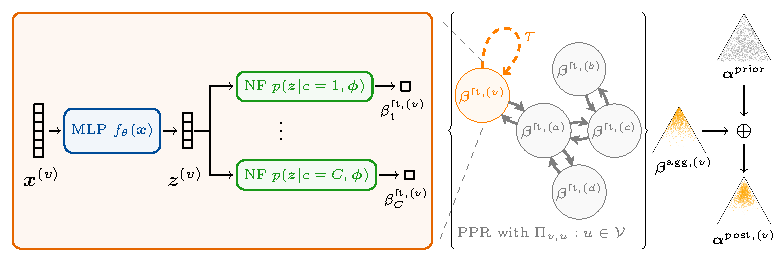
\includegraphics[width=.75\textwidth]{sections/009_neurips2021/resources/model.pdf}
	\caption{Overview of \GPN{}: (1) node-level pseudo-counts computed by the feature encoder in the orange box, (2) PPR-based message passing visualized between the curly braces, and (3) input-dependent Bayesian update illustrated with the Dirichlet triangles on the right.}
    \label{fig:model_vis}
    \vspace{-3mm}
\end{figure}

\looseness=-1
For classification, the predicted categorical distribution \smash{$\hat{\y} \nodeidxv \sim \DCat(\p\nodeidxv)$} additionally depends on the specific input $\nodev$. Hence, the \emph{input-dependent} Bayesian rule \citep{charpentier2020, NatPN2021} extends the Bayesian treatment of a single categorical distribution to classification by predicting an individual posterior update for any possible input. Specifically, it first introduces a fixed Dirichlet prior over the categorical distribution \smash{$\p\nodeidxv \sim \DDir(\valpha^\text{prior})$} where \smash{$\valpha^\text{prior} \in \real_+^\nclass$} is usually set to $1$, and second predicts the input-dependent update \smash{$\vbeta\nodeidxv$} which forms the posterior distribution \smash{$\p\nodeidxv \sim \DDir(\valpha^{\text{post}, (\nodev)})$} where the posterior parameters are equal to
\begin{align}\label{eq:input-posterior-update}
    \valpha^{\text{post}, (\nodev)} = \valpha^\text{prior} + \vbeta\nodeidxv.
\end{align}
The variable $\vbeta\nodeidxv$ can be interpreted as learned class pseudo-counts and its parametrization is crucial. For i.i.d. inputs, PostNet \citep{charpentier2020} models the pseudo-counts $\vbeta\nodeidxv$ in two main steps. \textbf{(1)} it maps the inputs features $\x\nodeidxv$ onto a low-dimensional latent vector \smash{$\z\nodeidxv= f_\theta(\x\nodeidxv) \in \real^H$}. \textbf{(2)}, it fits one conditional probability density \smash{$\prob(\z\nodeidxv|\iclass; \vphi)$} per class on this latent space with normalizing flows. The final pseudo count for class $c$ is set proportional to its respective conditional density i.e. \smash{$\beta_\iclass\nodeidxv = N \prob(\z\nodeidxv|\iclass; \vphi) \prob(\iclass)$} where $N$ is a total certainty budget and $\prob(\iclass)= \frac{1}{\nclass}$ for balanced classes. Note that this implies \smash{$\alpha_0\nodeidxv = N \prob(\z\nodeidxv|\vphi)$}. This architecture has the advantage of decreasing the evidence outside the known distribution when increasing the evidence inside the known distribution, thus leading to consistent uncertainty estimation far from training data.

\paragraph{Bayesian Update for Interdependent Inputs.} We propose a simple yet efficient modification for parameterizing $\beta_\iclass\nodeidxv$ to extend the input-dependent Bayesian update for interdependent attributed nodes. The core idea is to first predict the feature class pseudo-counts $\vbeta^{\text{ft}, (\nodev)}$ based on independent node features only, and then diffuse them to form the aggregated class pseudo-counts $\vbeta^{\text{agg}, (\nodev)}$ based on neighborhood features. Hence, the feature class pseudo-counts $\vbeta^{\text{ft}, (\nodev)}$ intuitively act as uncertainty estimates without network effects while the aggregated class pseudo-counts $\vbeta^{\text{agg}, (\nodev)}$ intuitively act as uncertainty estimates with network effects. 

\looseness=-1
To this end, \GPNacro{} performs three main steps (see \cref{fig:model_vis}). \textbf{(1)} A (feature) encoder maps the features of $\nodev$ onto a low-dimensional latent representation $\z$ i.e. $\z^{(\nodev)} = f_\theta(\x\nodeidxv) \in \real^H$. In practice, we use a simple MLP encoder in our experiments similarly to APPNP \citep{Klicpera2018}. \textbf{(2)} One conditional probability density per class \smash{$\prob(\z^{(\nodev)} \condition \iclass; \vphi)$} is used to compute \smash{$\beta_\iclass^{\text{ft}, (\nodev)}$} i.e \smash{$\beta_\iclass^{\text{ft}, (\nodev)} \propto \prob(\z^{(\nodev)} \condition \iclass; \vphi)$}. Note that the the total feature evidence \smash{$\alpha_0^{\text{ft}, (\nodev)}= \sum_\iclass \beta_\iclass^{\text{ft}, (\nodev)}$} and the parameter \smash{$\bar{\vp}^{\text{ft}, (\nodev)} = \nicefrac{\vbeta^{\text{ft}, (\nodev)}}{\alpha_0^{\text{ft}, (\nodev)}}$} are only based on node features and can be seen as epistemic and aleatoric uncertainty measures \emph{without network effects}. In practice, we used radial normalizing flows for density estimation similarly to \citep{charpentier2020} and scaled the certainty $N$ budget w.r.t. the latent dimension $H$ similarly to \citep{NatPN2021}. \textbf{(3)} A Personalized Page Rank (PPR) message passing scheme is used to diffuse the feature class pseudo-counts \smash{$\beta_\iclass^{\text{ft}, (\nodev)}$} and form the aggregated class pseudo-counts \smash{$\beta_\iclass^{\text{agg}, (\nodev)}$} i.e.
\begin{equation}\label{eq:agg-evidence}
    \beta_\iclass^{\text{agg}, (\nodev)} = \sum_{\nodeu \in \vertices} \pprelem_{v, u} \beta_\iclass^{\text{ft}, (\nodeu)}
\end{equation}
\looseness=-1
where $\pprelem_{v, u}$ are the dense PPR scores implicitly reflecting the importance of node $\nodeu$ on $\nodev$. We approximate the dense PPR scores using power iteration similarly to \citep{Klicpera2018}. The aggregated pseudo-count \smash{$\beta_\iclass^{\text{agg}, (\nodev)}$} is then used in the input-dependent Bayesian update (see \cref{eq:input-posterior-update}). Remark that the scores \smash{$\pprelem_{v, u}$} define a valid conditional distribution over all nodes associated to the PPR random walk (i.e. \smash{$\sum_\nodeu \pprelem_{v, u} = 1$}). It can be viewed as a soft neighborhood for $\nodev$ accounting for all neighborhood hops through infinitely many message passing steps \citep{Klicpera2018}. Hence, on one hand, the PPR scores define a probability distribution over nodes using the node edges only. On the other hand, the quantity \smash{$\prob(\z^{(\nodeu)} \condition \iclass; \vphi)$} defines a probability distribution over nodes using the node features only. Therefore, we can equivalently rewrite this step using probabilistic notations \smash{$\prob(\nodev \condition \nodeu) = \pprelem_{v, u}$} and \smash{$\prob(\nodeu \condition \iclass) = \prob(\z^{(\nodeu)} \condition \iclass; \vphi)$}:
\begin{equation}\label{eq:agg-evidence-density}
    \beta_\iclass^{\text{agg}, (\nodev)} \propto \bar{\prob}(\nodev \condition \iclass) = \sum_{\nodeu \in \vertices} \prob(\nodev \condition \nodeu) \prob(\nodeu \condition \iclass)
\end{equation}
\looseness=-1
Interestingly, the quantity $\bar{\prob}(\nodev \condition \iclass)$ defines a valid distribution which normalizes over all node features and accounts for the soft neighborhood (i.e. $\int...\int\bar{\prob}(\nodev \condition \iclass) d\z^{(u_1)}...d\z^{(u_{|\vertices|})} = 1$). Hence, the message passing step is a simple but efficient method to transform the feature distributions of a single node into a joint distributions over the soft neighborhood features. Finally, the evidence $\alpha_0^{\text{agg}, (\nodev)} = \sum_\iclass \beta_\iclass^{\text{agg}, (\nodev)}$ and the parameter $\vp^{\text{agg}, (\nodev)} = \nicefrac{\vbeta^{\text{agg}, (\nodev)}}{\alpha_0^{\text{agg}, (\nodev)}}$ are based on neighborhood features and can be seen as epistemic and aleatoric uncertainty measures \emph{with network effects}. Remark that, the sequential processing of the features (i.e. steps (1)+(2)) and network information (i.e. step (3)) in \GPNacro{} is a key element to differentiate between the uncertainty without and with network effects and is a building block to provably obey the desiderata.

\GPNacro{} extends both APPNP \cite{Klicpera2018} and PostNet \cite{charpentier2020} approaches. The key difference to APPNP is the density estimation modeling the epistemic uncertainty (i.e. steps (1)+(2)) and the input-dependent Bayesian update allowing to recover the prior prediction (i.e. \cref{eq:input-posterior-update}). The key difference to PostNet is the PPR diffusion which accounts for dependence between nodes (step (3)).

\paragraph{Optimization.} We follow \cite{charpentier2020} and train \GPNacro{} by minimizing the following Bayesian loss with two terms i.e.:
\begin{equation}
    \loss\nodeidxv = -\ExpecationArgs{\p\nodeidxv\sim \prior\namednodeidxv{post}}{\log \prob(\y\nodeidxv \condition \p\nodeidxv)} - \lambda \entropy{\prior\namednodeidxv{post}}
\end{equation}
where $\lambda$ is a regularization factor. It can be computed quickly in closed-form and provides theoretical guarantees for optimal solutions \cite{charpentier2020}. All parameters of \GPNacro{} are trained jointly. Similarly to \cite{NatPN2021}, we also observed that "warm-up" training for the normalizing flows is helpful. 